\def\documentType{Protocol}
\def\mainLanguage{ngerman}

%%%%%%%%%%%%%%%%%%%%%%%%%%%%%%%%%%%%%%%%%%%%%%%%%%%%%%%%%%%%%
%   LaTeX-Template, Version 0.1                	  	        %
%   Author: 	Tom Mohr <https://tomo2403.de>              %
%   License: 	GNU General Public License v3.0				%
%   Updates: 	https://github.com/tomo2403/LaTeX-Templates %
%%%%%%%%%%%%%%%%%%%%%%%%%%%%%%%%%%%%%%%%%%%%%%%%%%%%%%%%%%%%%

% This comment is required for the VS Code plugin "LaTeX Workspace."
% Because this file contains the '\documentclass[...]{...}', it would otherwise
% be incorrectly considered a root file.
% !TeX root = ./V6/master.tex

\RequirePackage{xstring}

\makeatletter
	\@ifundefined{documentType}{%
		\errmessage{Provide a type for document!} %
		\stop %
	}
	\@ifundefined{mainLanguage}{%
		\errmessage{Set the document language!} %
		\stop %
	}
\makeatother

\IfStrEqCase{\documentType}{
	{Protocol}{\documentclass[12pt,\mainLanguage,openany,numbers=noenddot,listof=totoc,bibliography=totoc,oneside]{scrbook}}%
	{Assignment}{\documentclass[a4paper,12pt,\mainLanguage,oneside]{scrartcl}}%
}[\errmessage{Unknown type: \documentType}\stop]


% =====================================================
%    Packages
% =====================================================

\usepackage{pgfkeys}
\usepackage{lastpage}

\usepackage{ifthen}
\usepackage{etoolbox}

\usepackage[utf8]{inputenc}
\usepackage[main=\mainLanguage]{babel}

\usepackage{lipsum}
\usepackage{graphicx}
\usepackage[\mainLanguage]{varioref}
\usepackage{float}
\usepackage{wrapfig}

% Lade Pakete abhängig vom documentType.
\IfStrEqCase{\documentType}{
	{Protocol}{
		\usepackage[a4paper, includehead, includefoot, left=3.0cm, right=2.5cm, top=2.5cm, bottom=2cm]{geometry}
		\usepackage[hyphens]{url}
		\usepackage[pdftex,pdfborderstyle={/S/U/W 1}]{hyperref}
	}
	{Assignment}{
		\usepackage{fancyhdr}
		\usepackage[a4paper, left=2.0cm, right=2.0cm, top=2.5cm, bottom=2cm]{geometry}
		\usepackage[hyphens]{url}
		\usepackage[pdftex,pdfborderstyle={/S/U/W 1}]{hyperref}
		\let\chapter\section
	}
}


% =====================================================
%    Deklaration der Variablen
% =====================================================

\pgfqkeys{/TemplateVersion0}{
	properties/Authors/.initial					= {MyAuthor1&&MyAuthor2},
	properties/Title/.initial					= {MyTitel},
	properties/Subtitle/.initial				= {MySubtitle},
	properties/Institution/.initial				= {MyInstitution},
	properties/Group/.initial					= {MyGroup},
	properties/Versioning/.initial				= {false},
	misc/Date/Prefix/.initial					= {From: },
	misc/Page/CountPrefix/.initial				= {Pages: },
	misc/Group/Prefix/.initial					= {Group: },
	misc/Version/Prefix/.initial				= {Version: },
	Protocol/Comment/.initial					= {MyComment},
}

% =====================================================
%    Eigene Befehle
% =====================================================

\newcommand{\get}[1]{\pgfkeysvalueof{/TemplateVersion0/#1}}
\newcommand{\seperator}{\par\noindent\rule{\textwidth}{0.4pt}}
\newcommand{\seperateAuthors}[1]{\noindent\StrSubstitute{\get{properties/Authors}}{&&}{#1}}


% =====================================================
%    Generiere passende Titelseiten, Kopfzeilen etc.
% =====================================================

\title{\get{properties/Title}}
\author{\seperateAuthors{, }}

\addto\captionsngerman{\renewcommand{\figurename}{Abb.}}
\addto\captionsenglish{\renewcommand{\figurename}{Fig.}}

\newbool{useVersioning}
\setbool{useVersioning}{\get{properties/Versioning}}
\ifbool{useVersioning}{
	\usepackage{mVersion}
	\setVersion{\get{misc/Version/Prefix}}
	\increaseBuild
}{}

\AtBeginDocument{
 	\IfStrEqCase{\documentType}{
 		{Protocol}{
 			\begin{titlepage}
	 			\thispagestyle{empty}
	 			\vspace*{4em}
	 			\begin{center}
%	 				\includegraphics[width=0.4\textwidth]{logo.jpg}\par
%	 				\vspace{1cm}

	 				\Huge\textbf{\get{properties/Title}}\par
	 				\vspace*{.5em}{\large\textbf{\get{properties/Subtitle}}\par}
					\vfill

					\small
	 				\ifthenelse{\equal{\get{Protocol/Comment}}{}}{}{{\em\vspace*{1em}\get{Protocol/Comment}\par}}
	 				\ifbool{useVersioning}{\version}{}\par
	 				\get{misc/Date/Prefix}\today\par
	 				\vspace*{1em}
	 				\vfill

	 				\Large\itshape\seperateAuthors{\par}
	 				\vfill
	 			\end{center}
 			\end{titlepage}

 			\pagenumbering{Roman}
 			\newpage
 			\tableofcontents
 			\newpage
 			\pagenumbering{arabic}
 		}
 		{Assignment}{
 			\setlength{\parindent}{0cm}

 			\fancypagestyle{firstPage}{
 				\setlength{\headheight}{75pt}
 				\fancyhf{}
 				\fancyhead[C]{
 					\seperateAuthors{, }\hfill{\get{misc/Group/Prefix}\get{properties/Group}} \\
 					\seperator

 					\noindent\textbf{\get{properties/Title}}\hfill{\textbf{\get{properties/Institution}}} \\
 					\noindent\emph{\get{properties/Subtitle}}
 					\hfill{Wintersemester 2024/2025}

 					\noindent\get{misc/Page/CountPrefix}\pageref*{LastPage}
 					\hfill{\get{misc/Date/Prefix}\today}
 				}
 				\fancyfoot[C]{
 					\thepage
 				}
 			}
 			\thispagestyle{firstPage}

			\fancypagestyle{defaultPage}{
				\setlength{\headheight}{29.5pt}
				\setlength{\textheight}{630pt}
				\fancyhf{}
				\fancyhead[L]{
					\textbf{\get{properties/Title}} \emph{(\get{properties/Subtitle})}\\\seperateAuthors{, }
				}
				\fancyhead[R]{
					\today\par\get{properties/Group}
				}
				\fancyfoot[C]{
					\thepage
				}
			}
 			\pagestyle{defaultPage}
 		}
 	}
}


\pgfqkeys{/TemplateVersion0}{
    properties/Authors 				= {Tom Mohr&&Martin Ohmeyer},
    properties/Title	 			= {Versuch V6},
    properties/Subtitle 			= {C405 Hardwarepraktikum II},
    properties/Institution 			= {HTWK Leipzig},
    properties/Group 				= {23INB-3},
    properties/Versioning 	      	        = {true},
    misc/Date/Prefix				= {Stand: },
    misc/Page/CountPrefix			= {Seiten: },
    misc/Group/Prefix				= {Gruppe: },
    Protocol/Comment		 	        = {Abnahme: 20. Januar 2025}
}

\usepackage{tikz}
\usepackage[table]{xcolor}
\usepackage[utf8]{inputenc}
\usepackage{color,soul}
\usepackage{mathtools}
\usepackage{transparent}
\usepackage{adjustbox}
\usepackage{tcolorbox}
\usepackage{inconsolata}
\usepackage{tabularx}
\usepackage{amsmath}
\usetikzlibrary{matrix}

\definecolor{darkgreen}{rgb}{0.0, 0.5, 0.0}

\usetikzlibrary{decorations.pathreplacing}
\usetikzlibrary{arrows, automata, positioning}
\graphicspath{{../images/}}

\begin{document}
        \chapter{Allgemeines}
\section{Zähler}
Variablen, die zu einem Zähler gehören, tragen die Bezeichnung $z_n$. 

\section{Würfel}
Variablen, die zum Würfel gehören, tragen die Bezeichnung $w_n$. Sie sind wie in Abbildung \ref{fig:dice} dargestellt auf die Augen des Würfels verteilt.
\vspace{2cm}
\begin{figure}[H]
    \centering
    \begin{tikzpicture}[scale=2.0]
        % Draw the dice outline
        \draw[thick] (0.3,0.3) rectangle (2.7,2.7);

        % Draw the dots
        % Group 1: Center dot
        \fill[blue, opacity=0.6] (1.5,1.5) circle (0.2); % Center dot

        % Group 2: Top-left and Bottom-right dots
        \fill[red, opacity=0.6] (0.75,2.25) circle (0.2); % Top-left dot
        \fill[red, opacity=0.6] (2.25,0.75) circle (0.2); % Bottom-right dot

        % Group 3: Bottom-left and Top-right dots
        \fill[darkgreen, opacity=0.6] (0.75,0.75) circle (0.2); % Bottom-left dot
        \fill[darkgreen, opacity=0.6] (2.25,2.25) circle (0.2); % Top-right dot

        % Group 4: Middle-left and Middle-right dots
        \fill[orange, opacity=0.6] (0.75,1.5) circle (0.2); % Middle-left dot
        \fill[orange, opacity=0.6] (2.25,1.5) circle (0.2); % Middle-right dot

        % Add colored and thick text to the right of the dice
        \node at (1.5, 0.0) {\textcolor{orange}{$w_3$} \ \textcolor{red}{$w_2$} \ \textcolor{darkgreen}{$w_1$} \ \textcolor{blue}{$w_0$}};
    \end{tikzpicture}
    \caption{Der Würfel}
    \label{fig:dice}
\end{figure}
        \chapter{Logikgatter}
\section{Wahrheitswerttabelle}

\begin{table}[H]
    \centering
    \def\arraystretch{1.3}
    \rowcolors{2}{gray!15}{white}
    \begin{tabular}{|c|c!{\vrule width 1.5pt}c|c|c!{\vrule width 1.5pt}c|c|c|c|}
        \rowcolor{gray!50}
        \hline
        Zähler & Würfel & $z_2$ & $z_1$ & $z_0$ & $w_3$ & $w_2$ & $w_1$ & $w_0$ \\
        \hline
        0      & 1      & 0     & 0     & 0     & 1     & 1     & 1     & 0     \\
        1      & 2      & 0     & 0     & 1     & 1     & 1     & 0     & 1     \\
        2      & 3      & 0     & 1     & 0     & 1     & 1     & 0     & 0     \\
        3      & 4      & 0     & 1     & 1     & 1     & 0     & 0     & 1     \\
        4      & 5      & 1     & 0     & 0     & 1     & 0     & 0     & 0     \\
        5      & 6      & 1     & 0     & 1     & 0     & 0     & 0     & 1     \\
        \hline
    \end{tabular}
    \caption{Mapping: Zähler auf Würfel}
    \label{tab:logicGates-truthtable}
\end{table}

\section{KV-Diagramme und vereinfachte Formeln}

\begin{table}[H]
    \centering
    \renewcommand{\arraystretch}{7.5}
    \begin{tabular}{c@{\hskip 1.5cm}c}
        \begin{tikzpicture}
            \matrix[matrix of nodes, nodes={draw, minimum size=1cm, anchor=center, text height=1.5ex, text depth=.25ex}] (kmap) {
            |[]| 1 & |[]| 1 & |[]| 1 & |[]| 1 \\
            |[]| 1 & |[]| 0 & |[]| x & |[]| x \\
            };

            % Add decimal numbers in the bottom right corner of each cell
            \foreach \i/\j/\num in {1/1/0, 1/2/1, 1/3/3, 1/4/2, 2/1/4, 2/2/5, 2/3/7, 2/4/6} {
                    \node[anchor=south east, font=\tiny] at (kmap-\i-\j.south east) {\num};
                }

            % Add variable names for columns
            \node[above=0.2cm of kmap-1-1.north] {$\overline{z}_0$};
            \node[above=0.2cm of kmap-1-2.north] {$z_0$};
            \node[above=0.2cm of kmap-1-3.north] {$z_0$};
            \node[above=0.2cm of kmap-1-4.north] {$\overline{z}_0$};

            % Add variable names for columns on the bottom
            \node[below=0.2cm of kmap-2-1.south] {$\overline{z}_1$};
            \node[below=0.2cm of kmap-2-2.south] {$\overline{z}_1$};
            \node[below=0.3cm of kmap-2-3.south] {$z_1$};
            \node[below=0.3cm of kmap-2-4.south] {$z_1$};

            % Add variable names for rows on the right
            \node[right=0.2cm of kmap-1-4.east] {$\overline{z}_2$};
            \node[right=0.2cm of kmap-2-4.east] {$z_2$};

            % Mark areas to simplify with multiple semi-transparent backgrounds
            \draw[fill=yellow, fill opacity=0.3, draw=none] (kmap-1-1.north west) rectangle (kmap-1-4.south east);

            \draw[fill=blue, fill opacity=0.3, draw=none] (kmap-1-1.north west) rectangle (kmap-2-1.south east);

            \draw[fill=blue, fill opacity=0.3, draw=none] (kmap-1-4.north west) rectangle (kmap-2-4.south east);

            \node[below=1cm of kmap] {$w_3 = \overline{z}_2 \ \lor \ \overline{z}_0$};
        \end{tikzpicture} &
        \begin{tikzpicture}
            \matrix[matrix of nodes, nodes={draw, minimum size=1cm, anchor=center, text height=1.5ex, text depth=.25ex}] (kmap) {
            |[]| 1 & |[]| 1 & |[]| 0 & |[]| 1 \\
            |[]| 0 & |[]| 0 & |[]| x & |[]| x \\
            };

            % Add decimal numbers in the bottom right corner of each cell
            \foreach \i/\j/\num in {1/1/0, 1/2/1, 1/3/3, 1/4/2, 2/1/4, 2/2/5, 2/3/7, 2/4/6} {
                    \node[anchor=south east, font=\tiny] at (kmap-\i-\j.south east) {\num};
                }

            % Add variable names for columns
            \node[above=0.2cm of kmap-1-1.north] {$\overline{z}_0$};
            \node[above=0.2cm of kmap-1-2.north] {$z_0$};
            \node[above=0.2cm of kmap-1-3.north] {$z_0$};
            \node[above=0.2cm of kmap-1-4.north] {$\overline{z}_0$};

            % Add variable names for columns on the bottom
            \node[below=0.2cm of kmap-2-1.south] {$\overline{z}_1$};
            \node[below=0.2cm of kmap-2-2.south] {$\overline{z}_1$};
            \node[below=0.3cm of kmap-2-3.south] {$z_1$};
            \node[below=0.3cm of kmap-2-4.south] {$z_1$};

            % Add variable names for rows on the right
            \node[right=0.2cm of kmap-1-4.east] {$\overline{z}_2$};
            \node[right=0.2cm of kmap-2-4.east] {$z_2$};

            % Mark areas to simplify with multiple semi-transparent backgrounds
            \draw[fill=yellow, fill opacity=0.3, draw=none] (kmap-1-1.north west) rectangle (kmap-1-2.south east);

            \draw[fill=blue, fill opacity=0.3, draw=none] (kmap-1-4.north west) rectangle (kmap-2-4.south east);

            \node[below=1cm of kmap] {$w_2 = \overline{z}_2 \overline{z}_1 \ \lor \ z_1 \overline{z}_0$};
        \end{tikzpicture}

        \\

        \begin{tikzpicture}
            \matrix[matrix of nodes, nodes={draw, minimum size=1cm, anchor=center, text height=1.5ex, text depth=.25ex}] (kmap) {
            |[]| 1 & |[]| 0 & |[]| 0 & |[]| 0 \\
            |[]| 0 & |[]| 0 & |[]| x & |[]| x \\
            };

            % Add decimal numbers in the bottom right corner of each cell
            \foreach \i/\j/\num in {1/1/0, 1/2/1, 1/3/3, 1/4/2, 2/1/4, 2/2/5, 2/3/7, 2/4/6} {
                    \node[anchor=south east, font=\tiny] at (kmap-\i-\j.south east) {\num};
                }

            % Add variable names for columns
            \node[above=0.2cm of kmap-1-1.north] {$\overline{z}_0$};
            \node[above=0.2cm of kmap-1-2.north] {$z_0$};
            \node[above=0.2cm of kmap-1-3.north] {$z_0$};
            \node[above=0.2cm of kmap-1-4.north] {$\overline{z}_0$};

            % Add variable names for columns on the bottom
            \node[below=0.2cm of kmap-2-1.south] {$\overline{z}_1$};
            \node[below=0.2cm of kmap-2-2.south] {$\overline{z}_1$};
            \node[below=0.3cm of kmap-2-3.south] {$z_1$};
            \node[below=0.3cm of kmap-2-4.south] {$z_1$};

            % Add variable names for rows on the right
            \node[right=0.2cm of kmap-1-4.east] {$\overline{z}_2$};
            \node[right=0.2cm of kmap-2-4.east] {$z_2$};

            % Mark areas to simplify with multiple semi-transparent backgrounds
            \draw[fill=yellow, fill opacity=0.3, draw=none] (kmap-1-1.north west) rectangle (kmap-1-1.south east);

            \node[below=1cm of kmap] {$w_1 = \overline{z}_2 \overline{z}_1 \overline{z}_0$};
        \end{tikzpicture} &
        \begin{tikzpicture}
            \matrix[matrix of nodes, nodes={draw, minimum size=1cm, anchor=center, text height=1.5ex, text depth=.25ex}] (kmap) {
            |[]| 0 & |[]| 1 & |[]| 1 & |[]| 0 \\
            |[]| 0 & |[]| 1 & |[]| x & |[]| x \\
            };

            % Add decimal numbers in the bottom right corner of each cell
            \foreach \i/\j/\num in {1/1/0, 1/2/1, 1/3/3, 1/4/2, 2/1/4, 2/2/5, 2/3/7, 2/4/6} {
                    \node[anchor=south east, font=\tiny] at (kmap-\i-\j.south east) {\num};
                }

            % Add variable names for columns
            \node[above=0.2cm of kmap-1-1.north] {$\overline{z}_0$};
            \node[above=0.2cm of kmap-1-2.north] {$z_0$};
            \node[above=0.2cm of kmap-1-3.north] {$z_0$};
            \node[above=0.2cm of kmap-1-4.north] {$\overline{z}_0$};

            % Add variable names for columns on the bottom
            \node[below=0.2cm of kmap-2-1.south] {$\overline{z}_1$};
            \node[below=0.2cm of kmap-2-2.south] {$\overline{z}_1$};
            \node[below=0.3cm of kmap-2-3.south] {$z_1$};
            \node[below=0.3cm of kmap-2-4.south] {$z_1$};

            % Add variable names for rows on the right
            \node[right=0.2cm of kmap-1-4.east] {$\overline{z}_2$};
            \node[right=0.2cm of kmap-2-4.east] {$z_2$};

            % Mark areas to simplify with multiple semi-transparent backgrounds
            \draw[fill=yellow, fill opacity=0.3, draw=none] (kmap-1-2.north west) rectangle (kmap-2-3.south east);

            \node[below=1cm of kmap] {$w_0 = z_0$};
        \end{tikzpicture}
    \end{tabular}
    \label{fig:logicGates-karnaugMaps}
\end{table}

\section{Aufbau}
\begin{figure}[H]
    \centering
    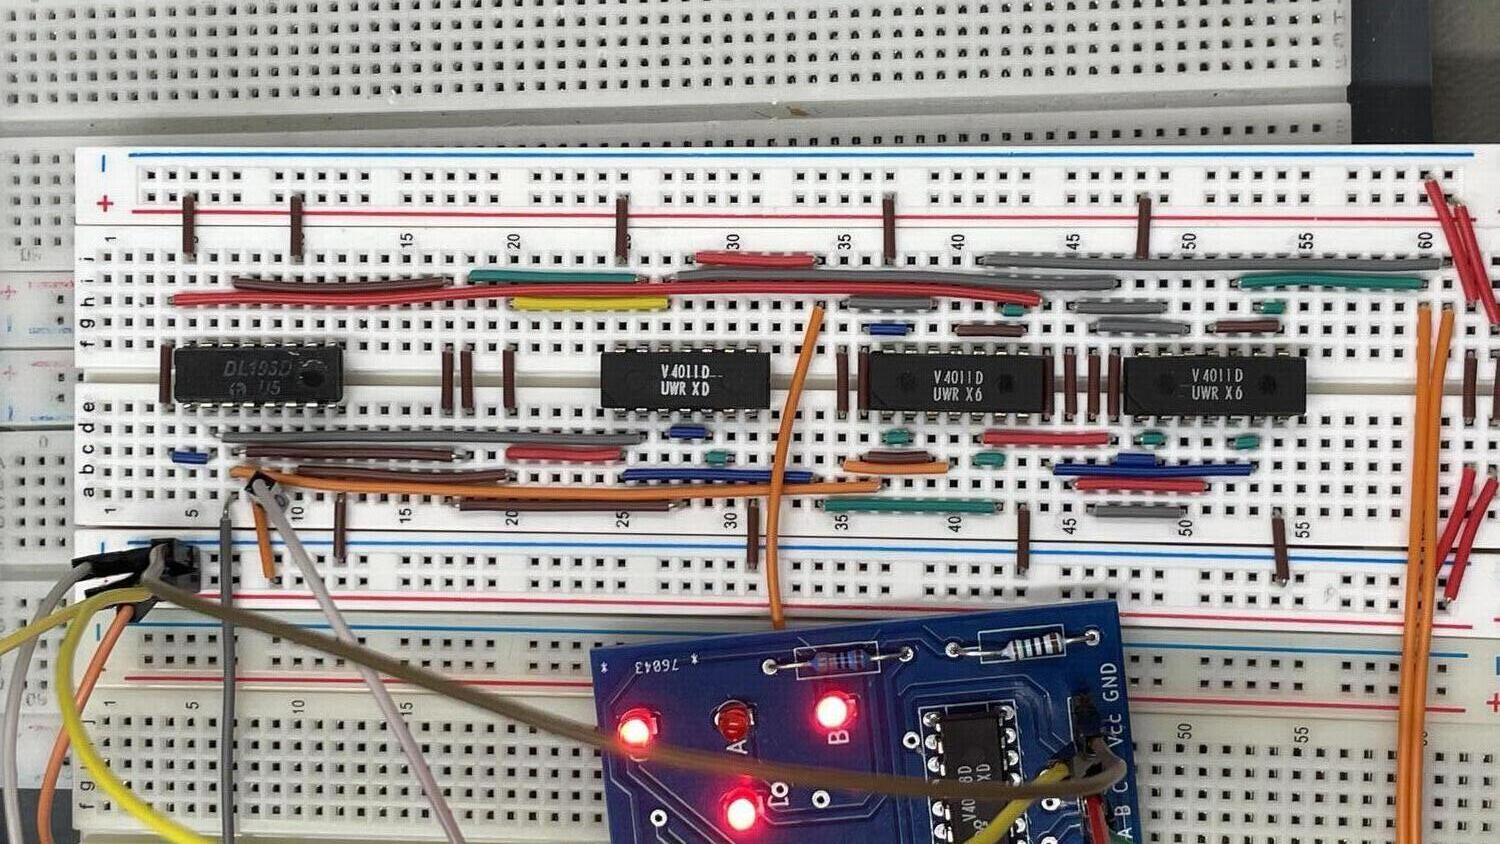
\includegraphics[width=0.8\textwidth]{dice_nand.jpeg}
    \caption{Aufbau der Schaltung mit 3 NAND-Gattern}
    \label{fig:logicGates-setup}
\end{figure}
\end{document}